\part{L'IHM générale de AIDA : \texttt{aito}}
\label{part:aito}


\texttt{aito} est l'interface générale de AIDA. Cette IHM permet d'accéder aux
acquisitions par naviguation dans les campagnes, dans les plateformes, dans les
acquisitions et par date. \\
Elle permet de lancer les principaux outils de AIDA qui seront décrits
\textbf{dans la suite de cette documentation}.


\section{Lancement}
\texttt{aito} doit être lancé en ligne de commande dans un terminal, par la
commande :

\fbox{ \texttt{aito} }


\section{Présentation}
La page principale de \texttt{aito} comporte plusieurs parties :

\begin{center}
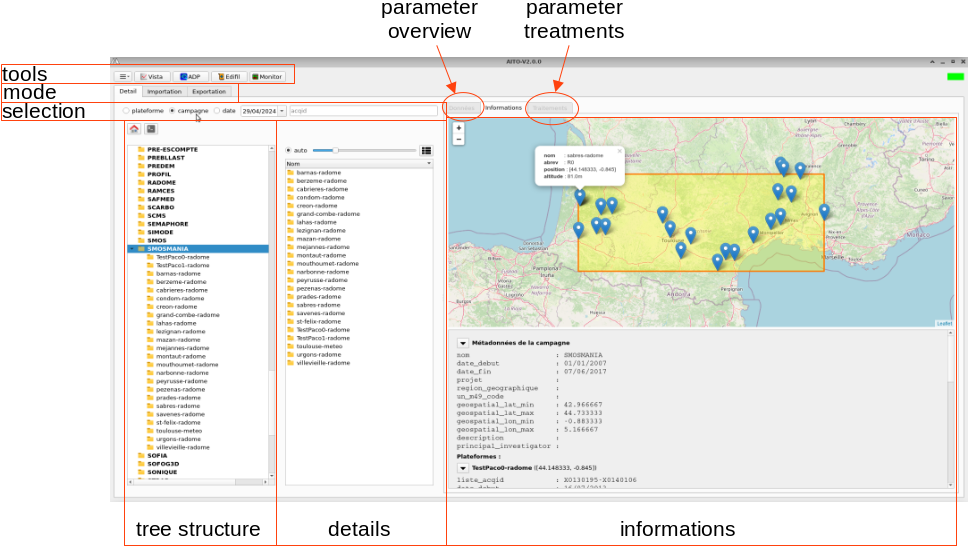
\includegraphics[width=14cm]{images/aito_main.png}
\end{center}

La partie supérieure donne accés, par des boutons, à différents outils de
AIDA (zone \texttt{tools}).

La zone \texttt{mode} permet de visualiser, d'importer et d'exporter des
données.

La zone \texttt{selection} permet de sélectionner le mode de navigation dans
les données (\texttt{plateforme}, \texttt{campagne}, \texttt{date},
\texttt{acqid}). Les zones \texttt{tree structure} et \texttt{detail} sont les
zones d'affichage de la navigation.

La partie droite est constituées de trois onglets (\texttt{information},
\texttt{données}, \texttt{traitements}). L'onglet \texttt{information} permet
de visualiser les informations sur l'objet sélectionné dans la partie
navigation. Lorsqu'un vecteur est sélectionné dans la partie naviagation, les
deux autres onglets (\texttt{données}, \texttt{traitements}) sont activés. \\

L'onglet \texttt{données} affiche les données du vecteur sous formes graphiques,
donne accés à quelques outils et informations concernant le vecteurs.

\begin{center}
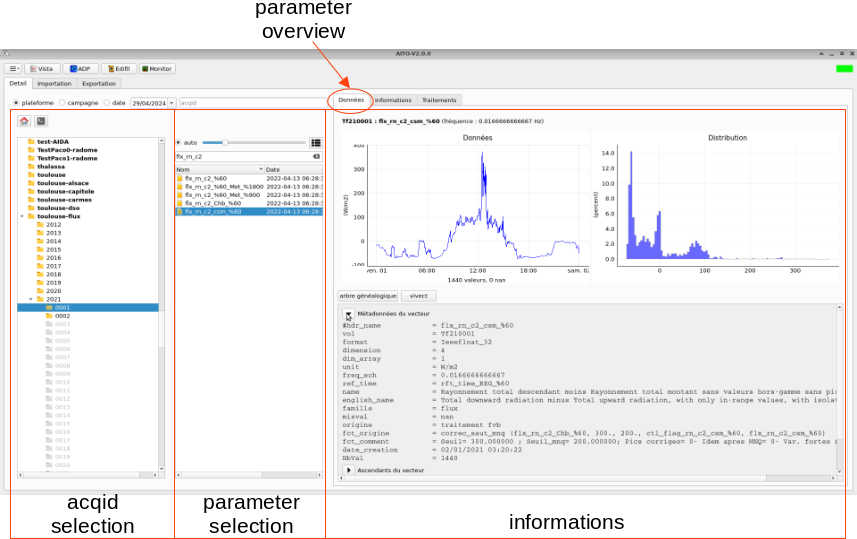
\includegraphics[width=14cm]{images/aito_vecteur_overview.png}
\end{center}

L'onglet \texttt{traitement} permet de visualiser le résultat de quelques
opérateur aux données du vecteur (le résultat des traitement n'est pas
enregistré sur disque).

\begin{center}
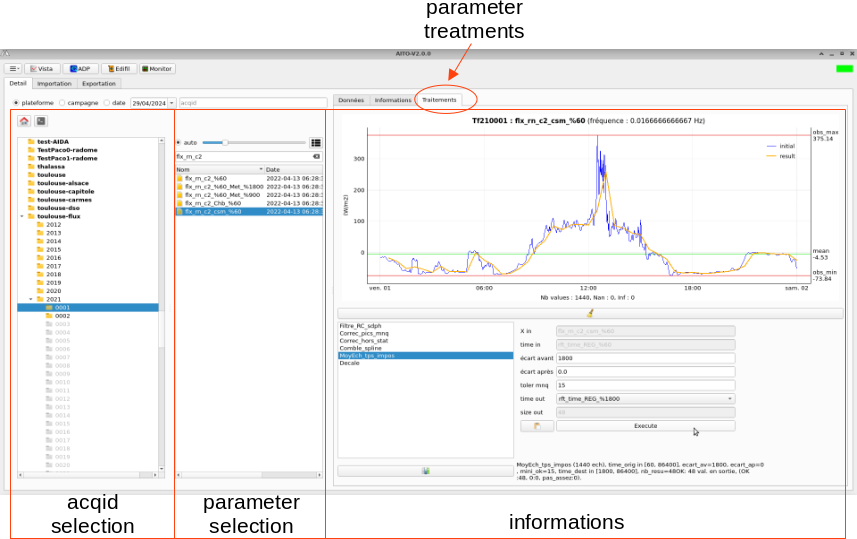
\includegraphics[width=14cm]{images/aito_vecteur_traitement.png}
\end{center}

